\documentclass[12pt]{article}

\usepackage{sbc-template}

\usepackage{graphicx,url}

\usepackage[brazil]{babel}   
%\usepackage[latin1]{inputenc}  
\usepackage[utf8]{inputenc}  
% UTF-8 encoding is recommended by ShareLaTex

     
\sloppy

\title{Exercício 5 - Laboratório de Redes de Computadores}

\author{Leonardo G. Carvalho\inst{1}, Matheus S. Redecker\inst{1}}


\address{Pontifícia Universidade Católica do Rio Grande do Sul - PUCRS
  \email{  \{leonardo.gubert\}\{matheus.redecker\} @acad.pucrs.br}
}

\begin{document} 

\maketitle


\section{}
\subitem{a)} Sim, podemos ver na figura \ref{1solicitation} que quem utiliza o comando ping 6 envia uma solicitação de "neighbor solicitation" para então achar o MAC da maquina que deseja fazer o ping, logo após é obtida uma mensagem de "neighbor advertisement" como pode ser visto na figura \ref{1advertisement}, onde uma outra maquina na rede responde com a informação do MAC.


\begin{figure}[ht]
\centering
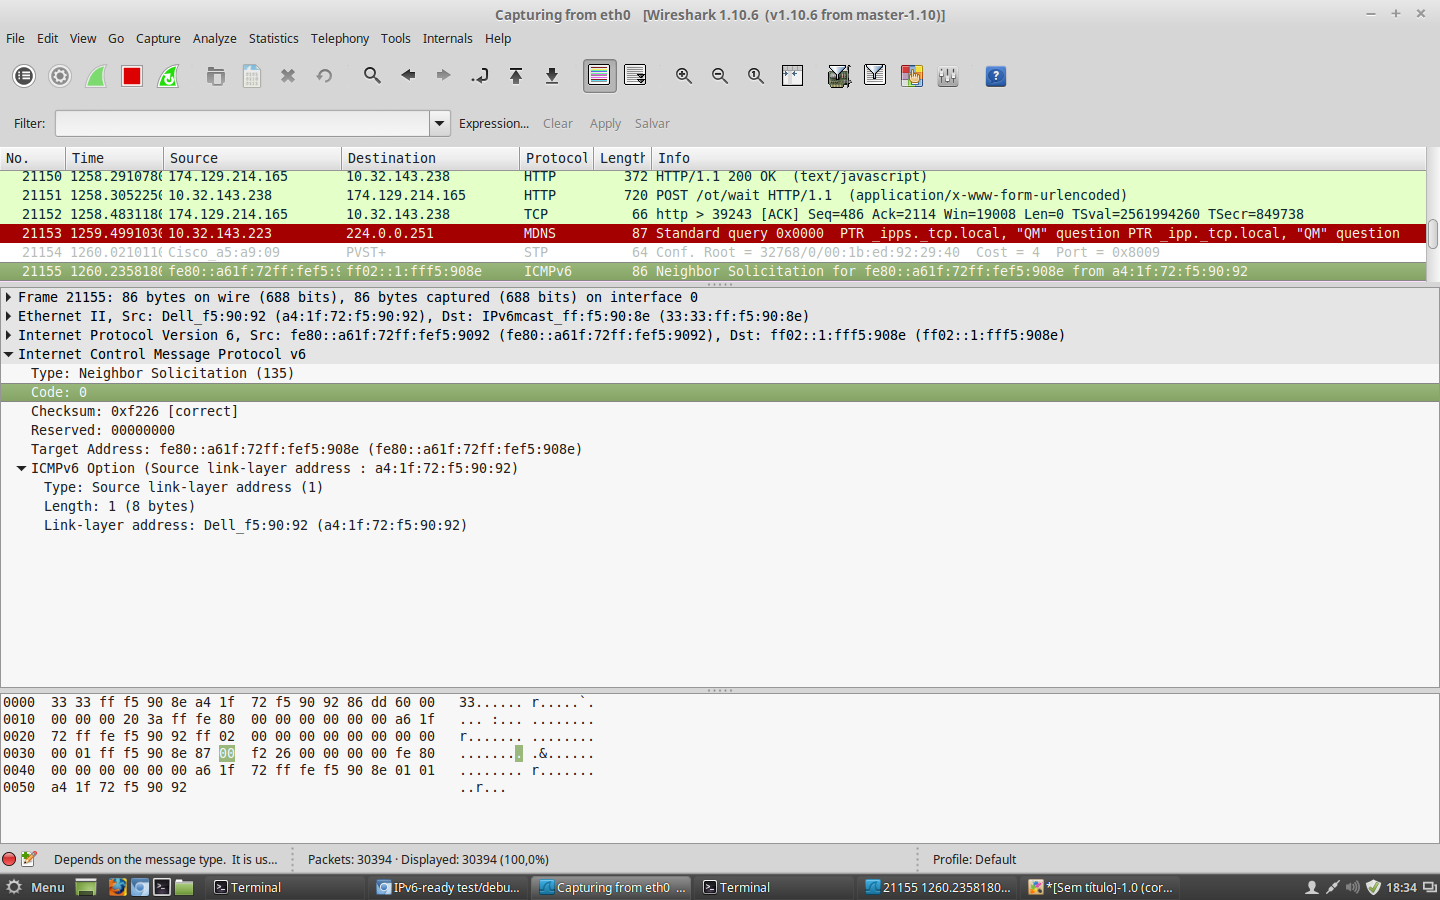
\includegraphics[scale=0.25]{neighborsolicitation.png}
\caption{Neighbor Solicitation}
\label{1solicitation}
\end{figure}

\newpage{}

\begin{figure}[ht]
\centering
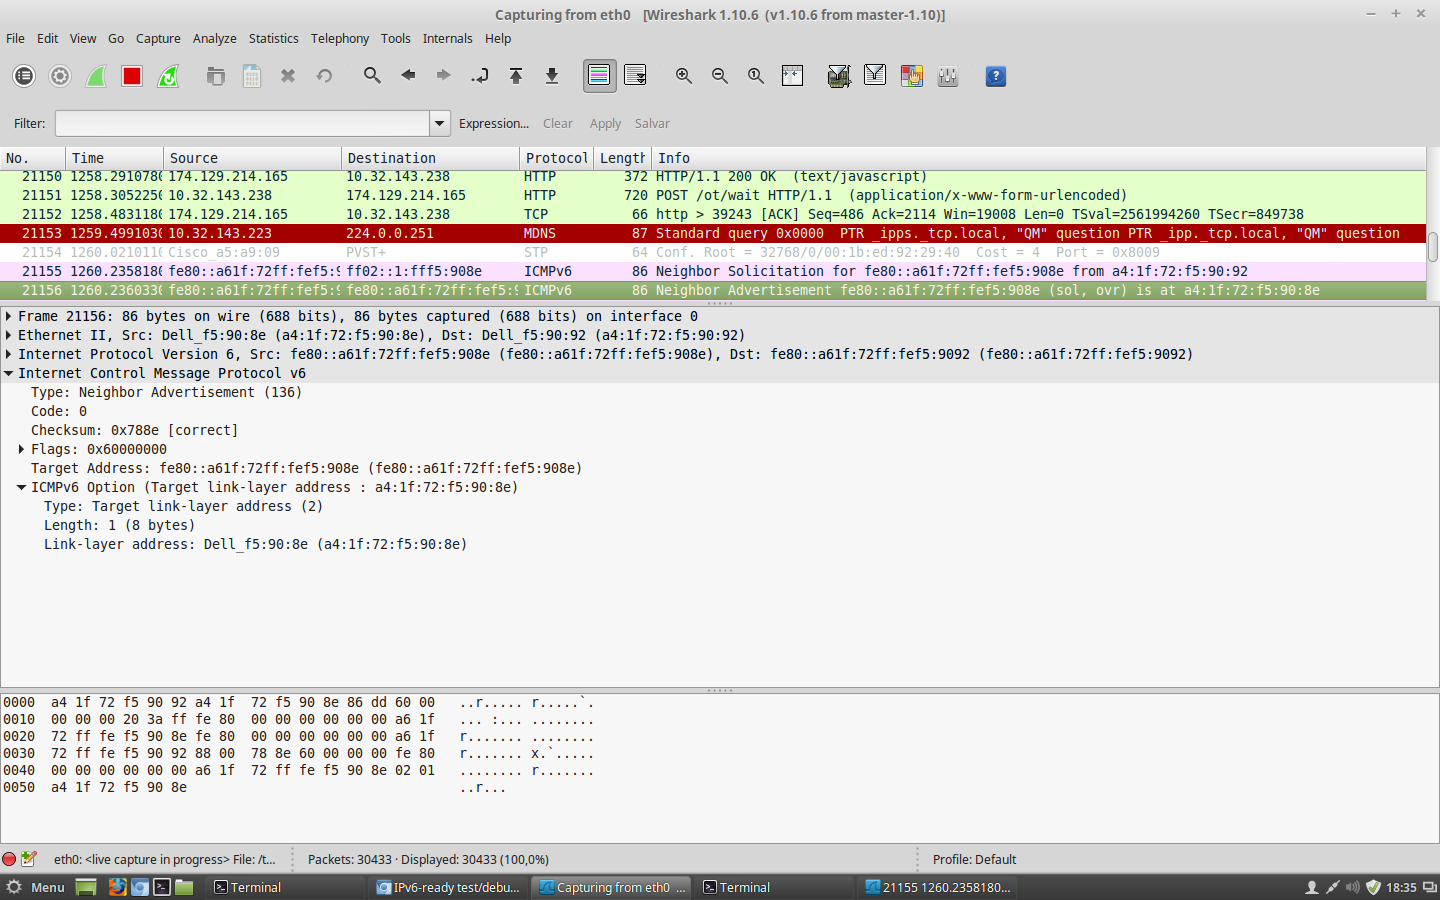
\includegraphics[scale=0.25]{neighboradvertisement.png}
\caption{Neighbor Advertisement}
\label{1advertisement}
\end{figure}



\subitem{b)} 
Com a utilização do comando obtemos as seguintes informações.
\begin{verbatim}
labredes-OptiPlex-3010 labredes #  ip -6 neigh show 
2001:db8:85a3::8a2e:370:7334 dev eth0 lladdr 50:3d:e5:d9:02:58 
router STALE
fe80::523d:e5ff:fed9:258 dev eth0 lladdr 50:3d:e5:d9:02:58 
router STALE
fe80::523d:e5ff:fe81:ede6 dev eth0 lladdr 50:3d:e5:81:ed:e6 
router STALE
fe80::523d:e5ff:fe81:ee4a dev eth0 lladdr 50:3d:e5:81:ee:4a 
router STALE
fe80::a61f:72ff:fef5:908e dev eth0 lladdr a4:1f:72:f5:90:8e STALE
\end{verbatim}

\subitem{c)}
Após a troca de mensagens para determinar o endereço MAC, as mensagens de echo request e echo reply são enviadas. Os cabeçalhos do IPv6 e do ICMPv6 são vistos nas figuras \ref{1request} e \ref{1reply}. 
\begin{figure}[ht]
\centering
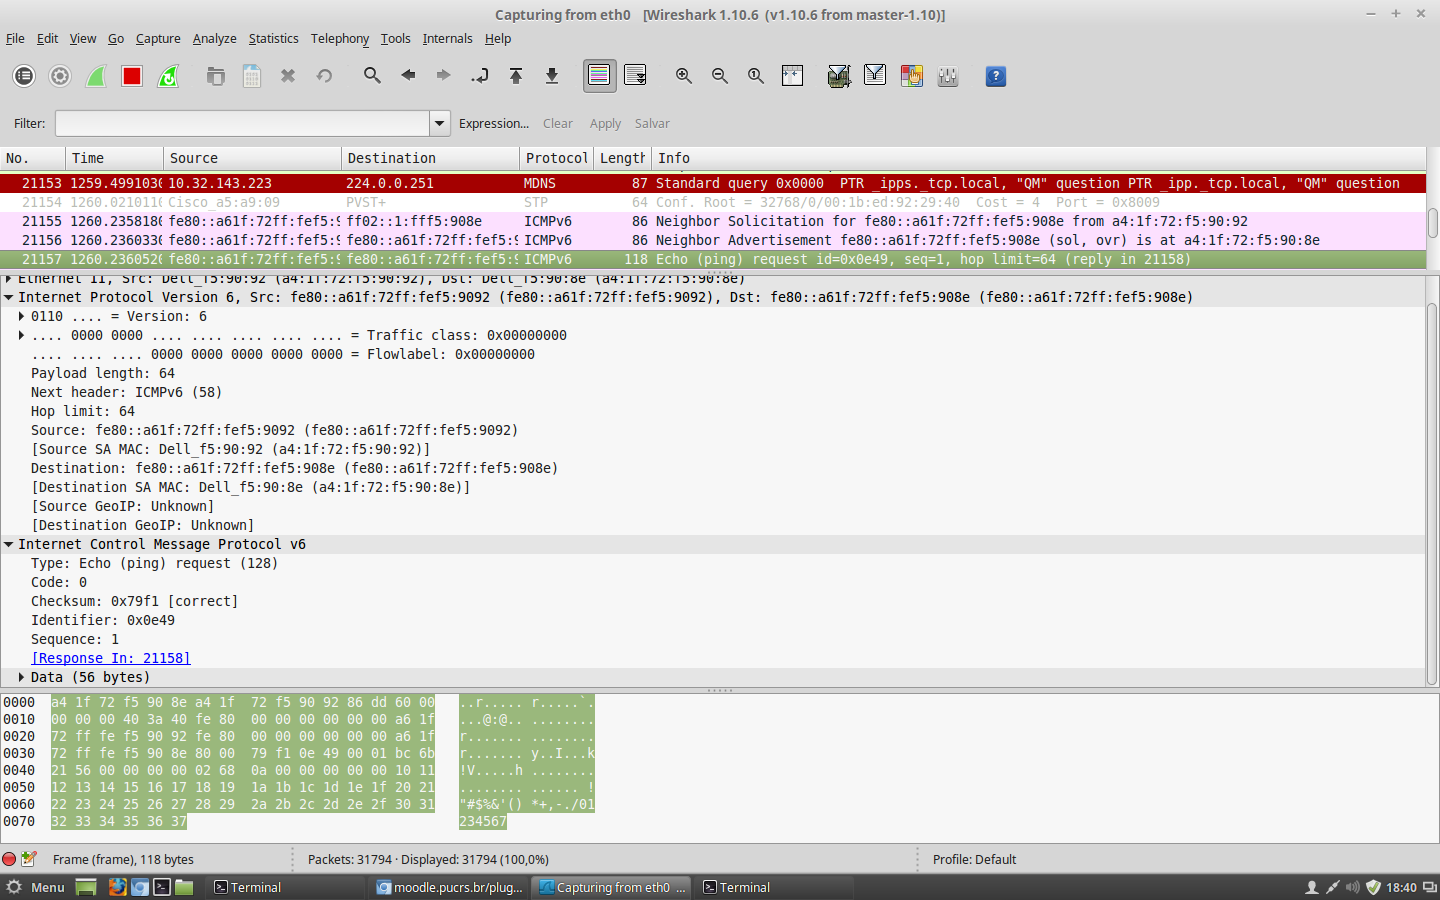
\includegraphics[scale=0.25]{request.png}
\caption{Echo Request}
\label{1request}
\end{figure}

\newpage{}
\begin{figure}[ht]
\centering
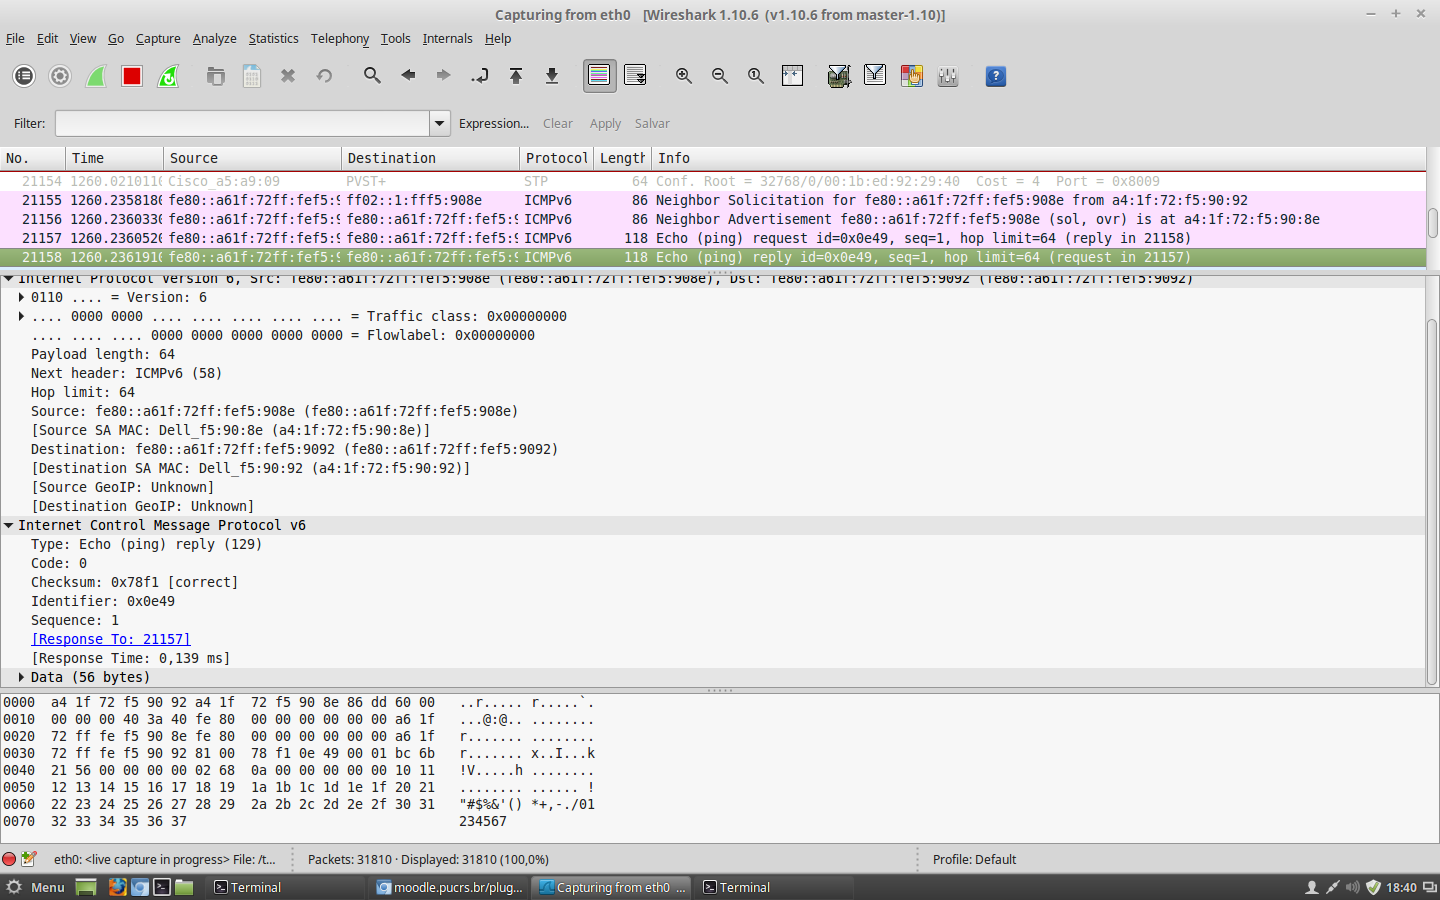
\includegraphics[scale=0.25]{reply.png}
\caption{Echo Reply}
\label{1reply}
\end{figure}

\section{}
Quando a maquina fica disponível novamente é enviado uma mensagem de "neighbor solicitation" para determinar o endereço do vizinho, essa mensagem também é usada para verificar se o vizinho ainda está alcançável via cache e ainda para ver se não existem duplicação de endereços. O IPv6 da maquina utilizada para a realização desse teste foi FE80:A61F:72FF:FEF5:908E e o conteúdo da mensagem pode ser visto na figura \ref{2}.

\begin{figure}[ht]
\centering
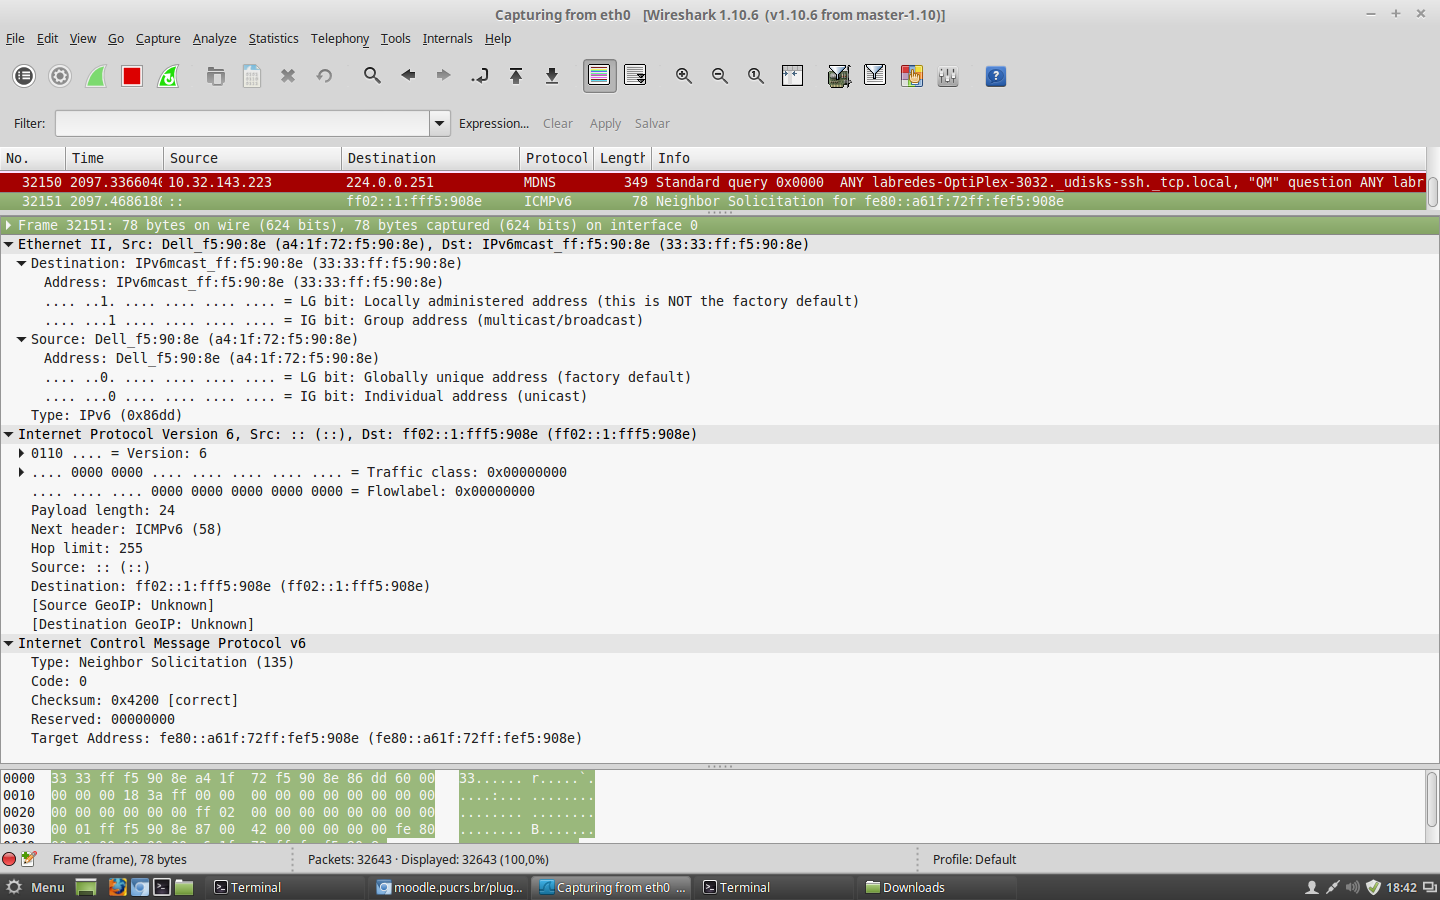
\includegraphics[scale=0.25]{dois.png}
\caption{}
\label{2}
\end{figure}

\section{}
Na figura \ref{3.1} podemos ver a mensagem quando o IPv6 da maquina é informado manualmente. Já quando colocamos o IPv6 igual ao da outra maquina ninguém ficou sem internet, pois a conexão está sendo feita pelo IPv4 e não o IPv6. Mas utilizando apenas os endereços IPv6, com a configuração do mesmo IP para as duas maquinas, as maquinas que estiverem com o endereço IP-MAC na cache irão se comunicar com a maquina certa, e a maquina que colocou o IPv6 de forma duplicada ficaria sem acesso a internet. O conteúdo das mensagens quando os IPs são iguais podem ser vistos nas figuras \ref{3soli} e \ref{3adver}.
\begin{figure}[ht]
\centering
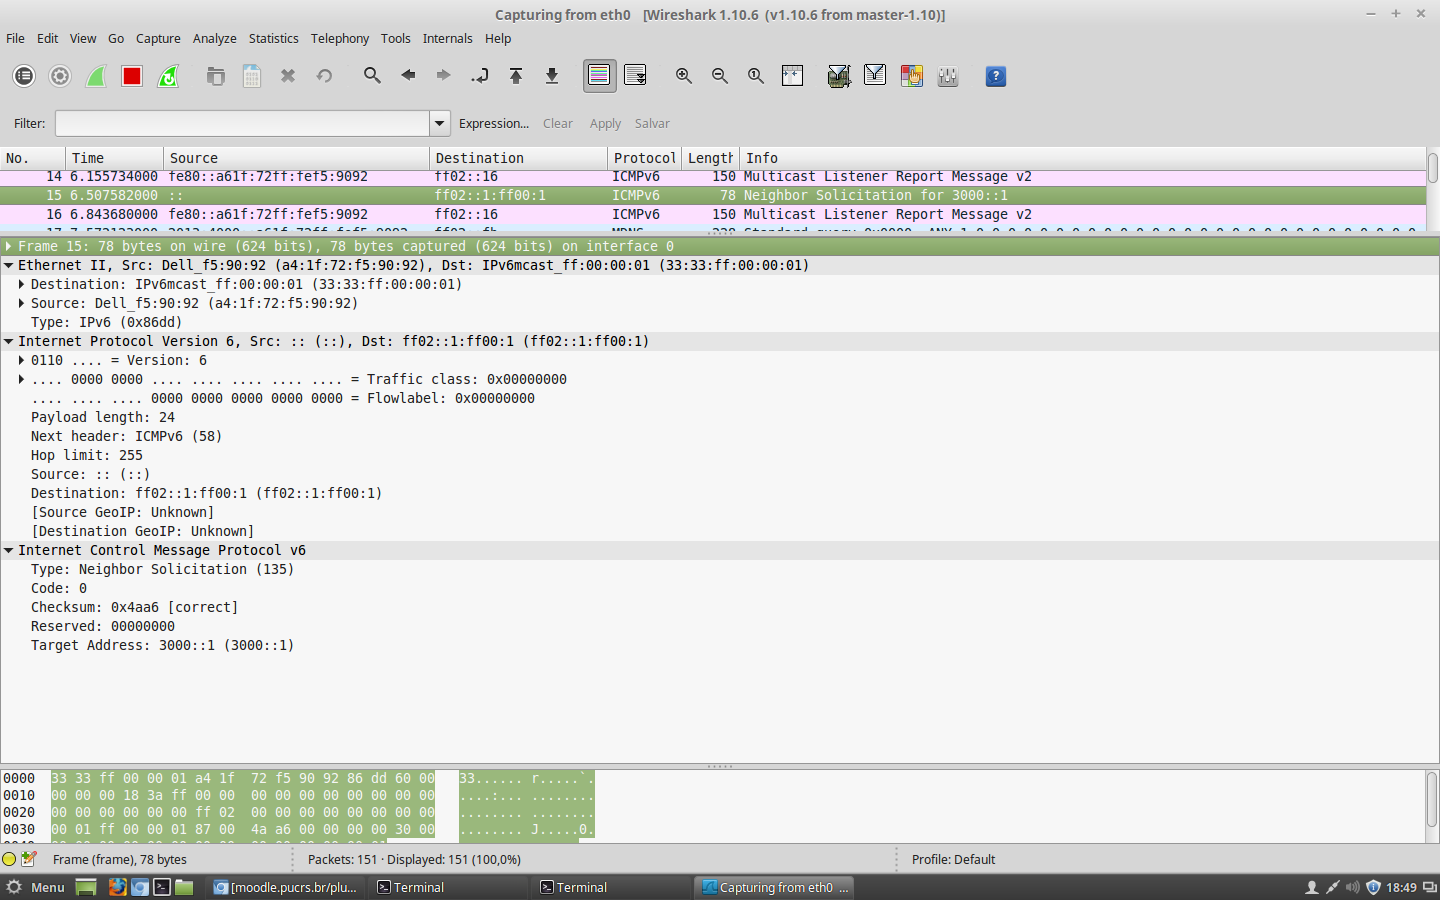
\includegraphics[scale=0.25]{teste1.png}
\caption{}
\label{3.1}
\end{figure}
\begin{figure}[ht]
\centering
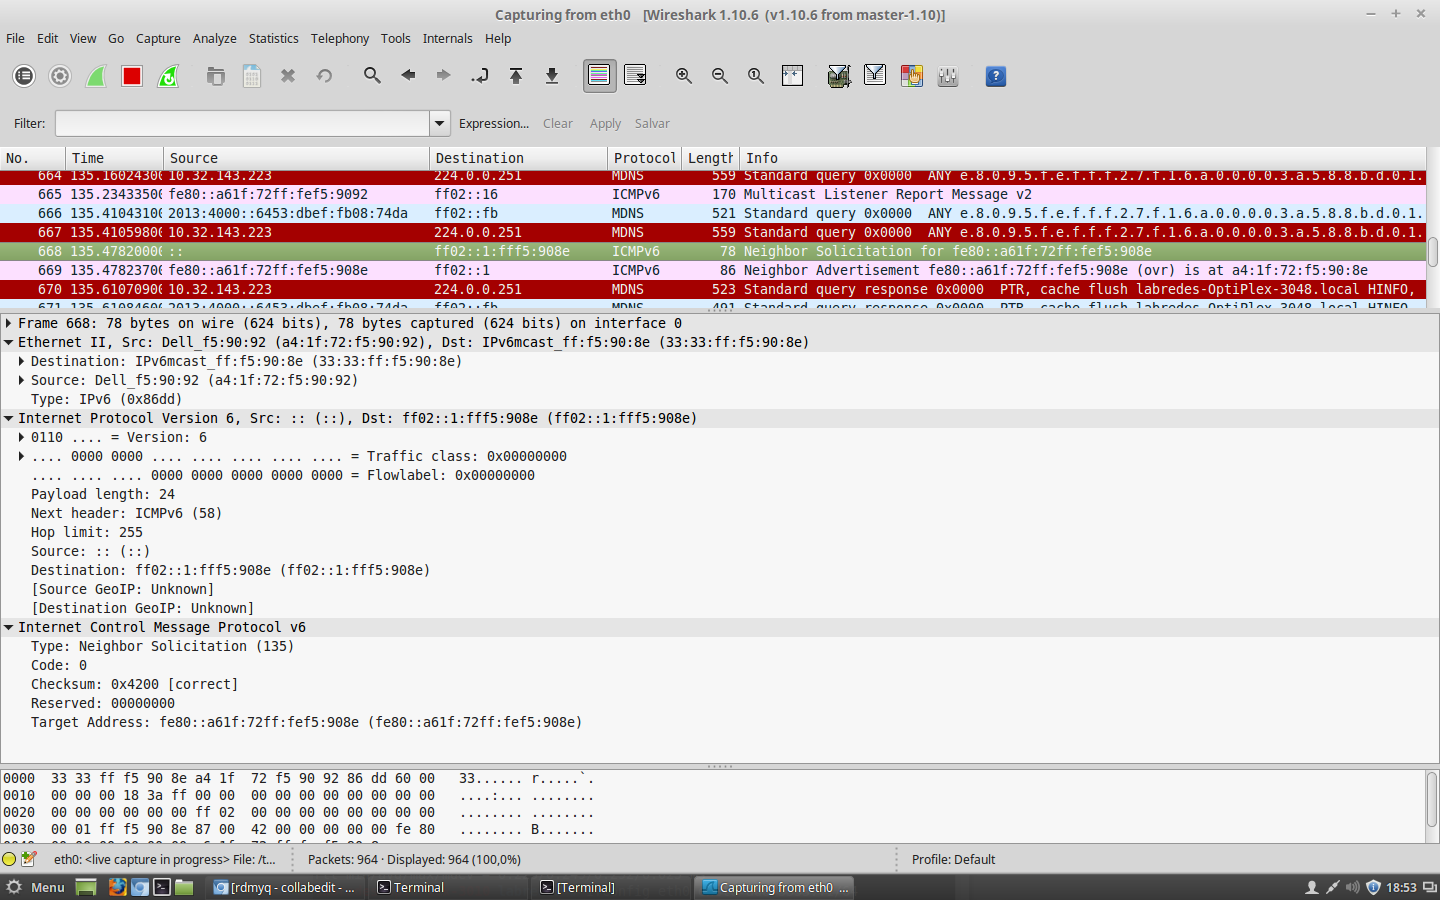
\includegraphics[scale=0.25]{neighborsolicitation3quandomatheuspegoumeuip.png}
\caption{}
\label{3soli}
\end{figure}
\begin{figure}[ht]
\centering
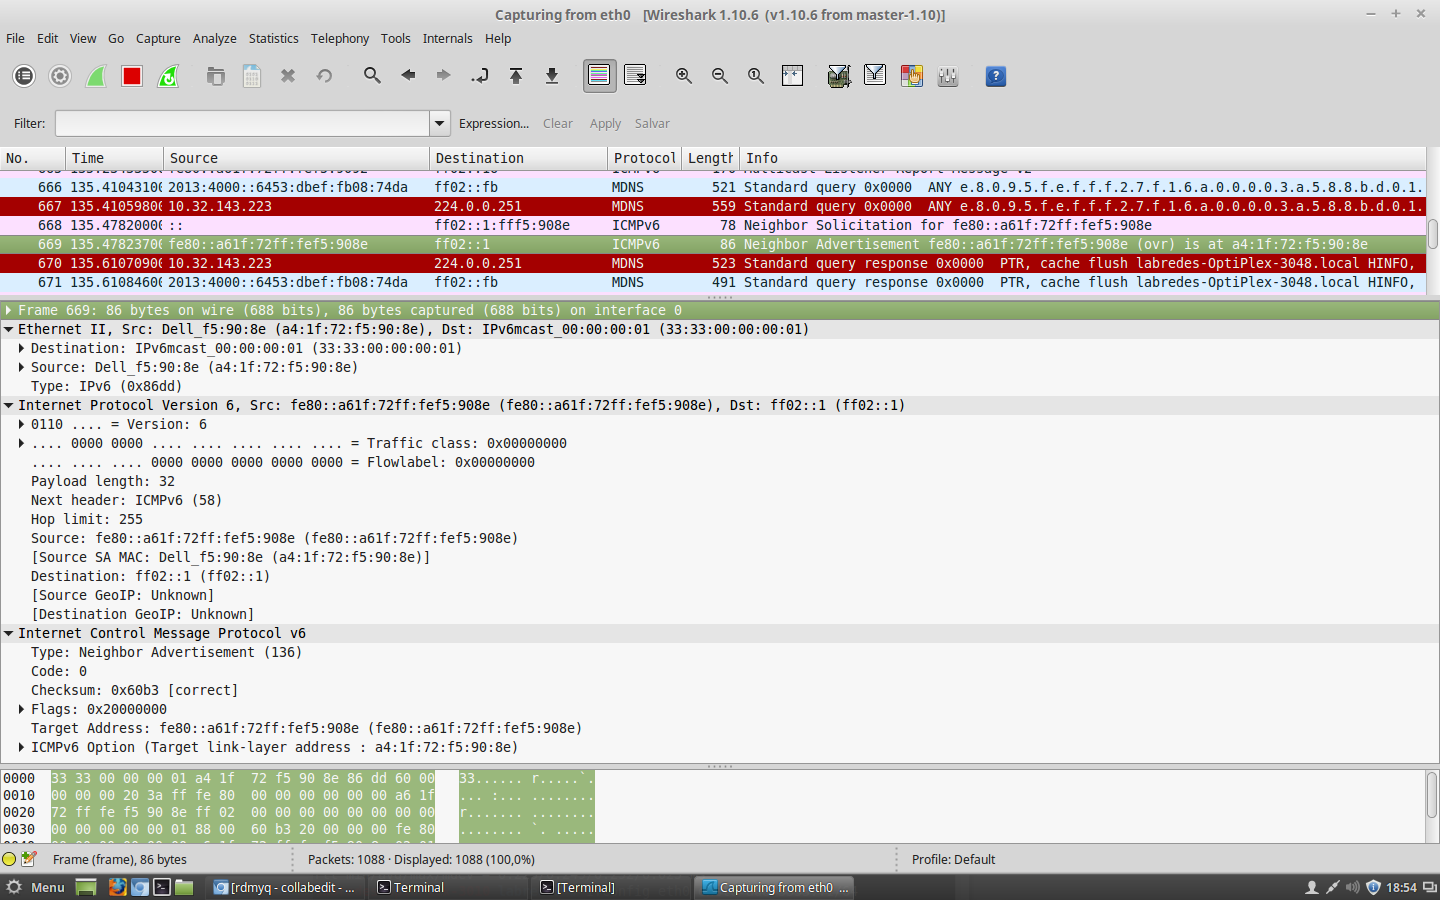
\includegraphics[scale=0.25]{neighboradvertisementquandoomatheuspegoumeuip.png}
\caption{}
\label{3adver}
\end{figure}

\end{document}
